\section{Edge Adding Algorithm}


\begin{figure}[ht]
\label{edge-add}
\centering
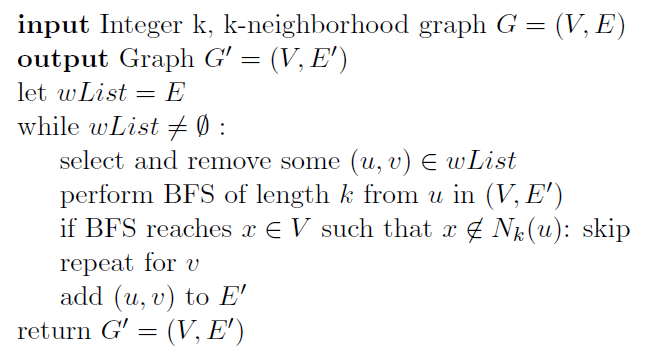
\includegraphics[scale=0.6]{Edge-Adding.png}
\caption{Pseudocode for the Edge-Adding Algorithm}
\label{fig:Edge-Adding Pseudocode}
\end{figure}


\indent The edge-adding algorithm, as shown in figure \ref{edge-add}, is a greedy algorithm which find a graph $G = (V,E)$ that approximately satify a given k-neighborhood graph, $G_k = (V, E')$. The algorithm works to find a graph whose k-neighborhood is at least a subgraph of $G_k$. It begins by adding the edges of $G_k$ into a working list. We know any satisfying graph must be a subgraph of $G_k$, as every edge of a graph must be included in the k-neighborhood of that graph. Therefore, we want to find a subset of our working list that satisfies $G_k$. This algorithm works by iteratively adding edges from the working list to the new graph.  At each iteration, a random edge $(u,v)$ is selected and removed from the working list. A breadth-first search of length $k$ is run from both $u$ and $v$ in the current graph, $G$. If the search (say, from $u$) reaches a node that is not adjacent to $u$ in $G_k$, then we know adding $(u,v)$ to $G$ would invalidate the graph and the edge is discarded. If no such node is found, then $(u,v)$ is added to $G$. This process continues until the working list is empty. This algorithm runs in $O(|E|*d^k)$ time, where $d$ is the maximum node density. As social networking graphs are typically sparse, this algorithm runs in near-linear time. 

\begin{figure}[ht]
\centering
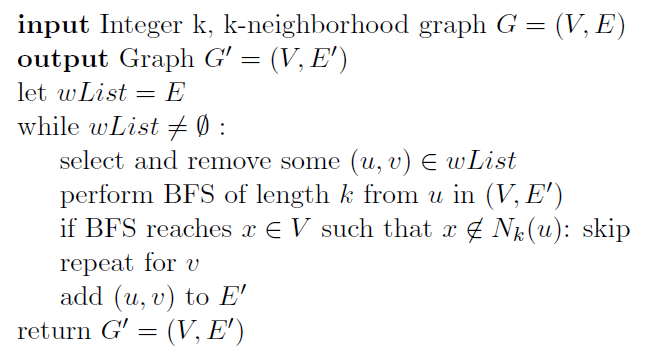
\includegraphics[scale=0.3 ]{Edge-Adding.png}
\caption{An example of the edge-adding algorithm. a) The 3-neighborhood graph for a given input. Each edge in this graph is added to the potential-edge list at the start of the algorithm. b) The solid lines represent edges that will be in the graph the algorithm returns (edge (B,D) was the last edge added). The dotted lines are remaining edges in the potential-edge list. After (B,D) was added, there became a 2-path between A and D. Since E is not adjacent to A in the 3-neighborhood graph, the edge (D,E) was removed from the potential-edge list.}
\label{fig:profs example}
\end{figure}